\chapter{Test af equalizer}\label{sec:test_eq}


\begin{figure}[h]
	\vspace*{-1 cm}
	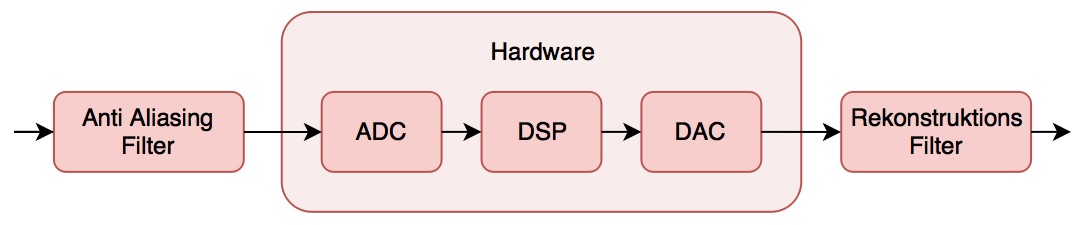
\includegraphics[width=8cm]{billeder/flow_all}
	\vspace{0.5 cm}
\end{figure}


\emph{I dette kapitel bliver der redegjort for testforløbet af equalizeren. Der bliver brugt en Bode 100 til måling af equalizerens overførselsfunktion. På denne måde kan det bevises om equalizerens profiler fungerer korrekt.}

\section{Forberedelse}


For bedst at teste equalizeren, blev der besluttet at følgende tre 3 parametre skulle gennemtestes: 

\begin{enumerate}[noitemsep,nolistsep]
    \item Amplituden/Gain
    \item Bandwidth
    \item Frekvens \\
\end{enumerate}



Under disse parametre var der en del forskellige ting der skulle tages højde for. 
\begin{enumerate}[noitemsep,nolistsep]
    \item Ved amplituden skulle der holdes en fast bandwidth ($100\hertz$) og en fast frekvens ($1\kilo\hertz$). Der blev målt hhv. $\pm5\decibel$ og $\pm7\decibel$
    \item Ved bandwidth skulle der holdes en fast amplitude ($\pm5\decibel$) samt en fast frekvens. ($1\kilo\hertz$). Her blev der målt forskellig bandwidth, hhv. $100\hertz$, $500\hertz$ og $1\kilo\hertz$.
    \item Ved frekvensen blev der holdt en fast amplitude ($\pm5\decibel$) og fast bandwidth ($100\hertz$). Her blev der dog målt med forskellige typer filtre. Peak filtret blev målt ved $100\hertz$ og $5\kilo\hertz$, hvor high shelf og low shelf filtrene blev målt ved $1\kilo\hertz$ og $5\kilo\hertz$. \\
\end{enumerate}

Derudover blev der opstillet en "kode-test" hvor der blev beregnet filtre som alle havde samme egenskaber, uanset om dette var et peak, high shelf eller et low shelf. Dette var for at eftervise om DSP koden var konsistent i alle typer filtre. \\

\section{Udførelse}
For at måle overføringsfunktionen sættes Bode 100'ens output til indgangen på equalizeren. CH1 sættes også til indgangen. CH2 sættes til udgangen og målingen foretages for samtlige af ovenstående presets. \\


\begin{figure}[h!]\label{fig:bode_setup}
	\centering
	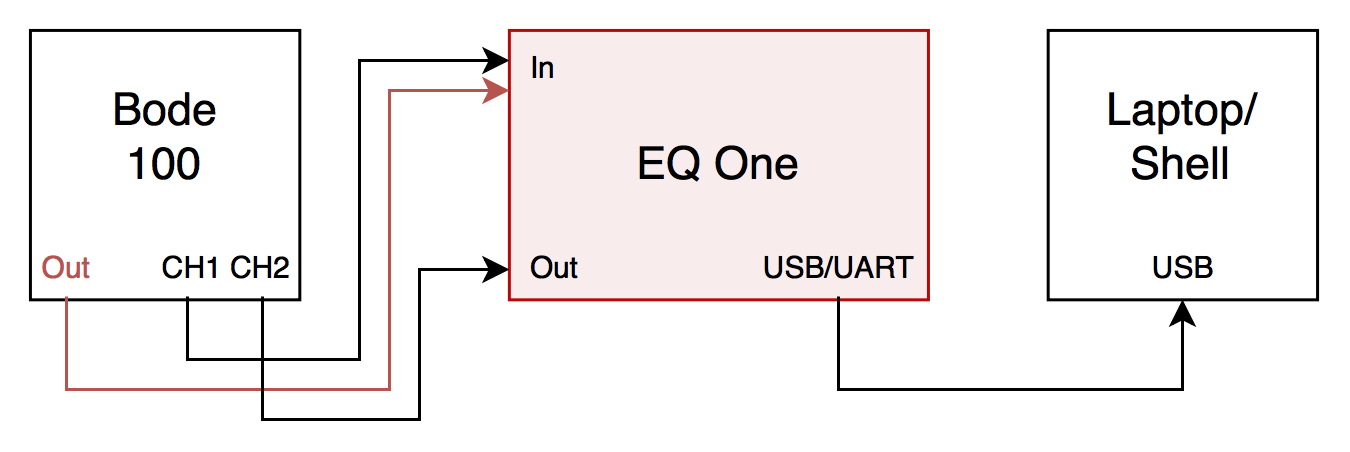
\includegraphics[width=13cm]{billeder/bode_setup}
	\caption{Målingssetup med Bode 100}
\end{figure}	

\FloatBlock

\section{Resultater}
I dette afsnit vil resultaterne af målingerne blive sammenlignet med de teoretiske udregninger og grafer.
Det første resultat på figur \ref{fig:eq_off1}, viser en graf hvor den digitale del er slået fra, og selve equalizeren er deaktiveret. Det er altså kun de analoge filtre der dominerer. Det teoretiske AA-filter ses til sammenligning på figur \ref{fig::afilter_aasim}. \\
Den vigtige del at eftervise, er hvor equalizeren er slået til. 






%Som det ses på figur \ref{fig:rock_test} ligger testresultaterne meget tæt på de teoretiske. Det vurderes at dette ligger inden for fejlmargin. Målingerne blev foretaget med et indgangssignal på 4dBm, for at sikre at ingen af profilerne overstyrede.


%\begin{figure}[h!]
%	\centering
%	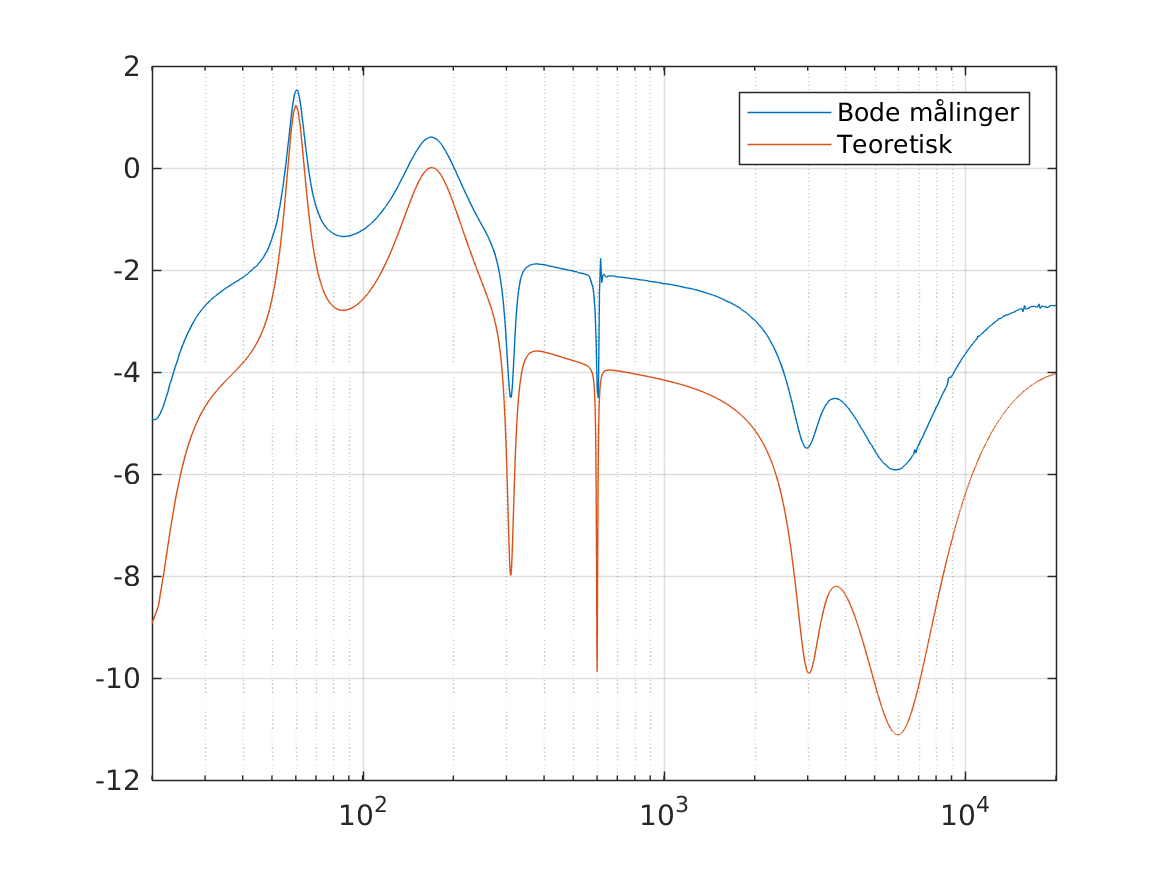
\includegraphics[width=15cm]{billeder/rock_test}
%	\caption{Sammenligning af "Rock"-profilen, teoretisk (orange) og måling (blå)}
%	\label{fig:rock_test}
%\end{figure}
	

%Der blev dog, vha. testene, fundet en fejl i DSP-beregningerne, som derfor kunne rettes. Der blev opdaget at den angivede frekvens i profilen altid var fordoblet på udgangen. Dette var på grund af at udregningen skulle ganges med $\frac{f_s}{2}$ i stedet for $f_s$. \\ 
%
%Det ses også at båndenes amplitude heller ikke stemmer helt overens. Dette kan skyldes indgang- og udgangsfiltrene eller en fejlberegning i DSP-koden. 
%
%
%\husk{SF}{Dette skal specificeres. Dennis? :D}




%\begin{figure}[h]
%\centering
%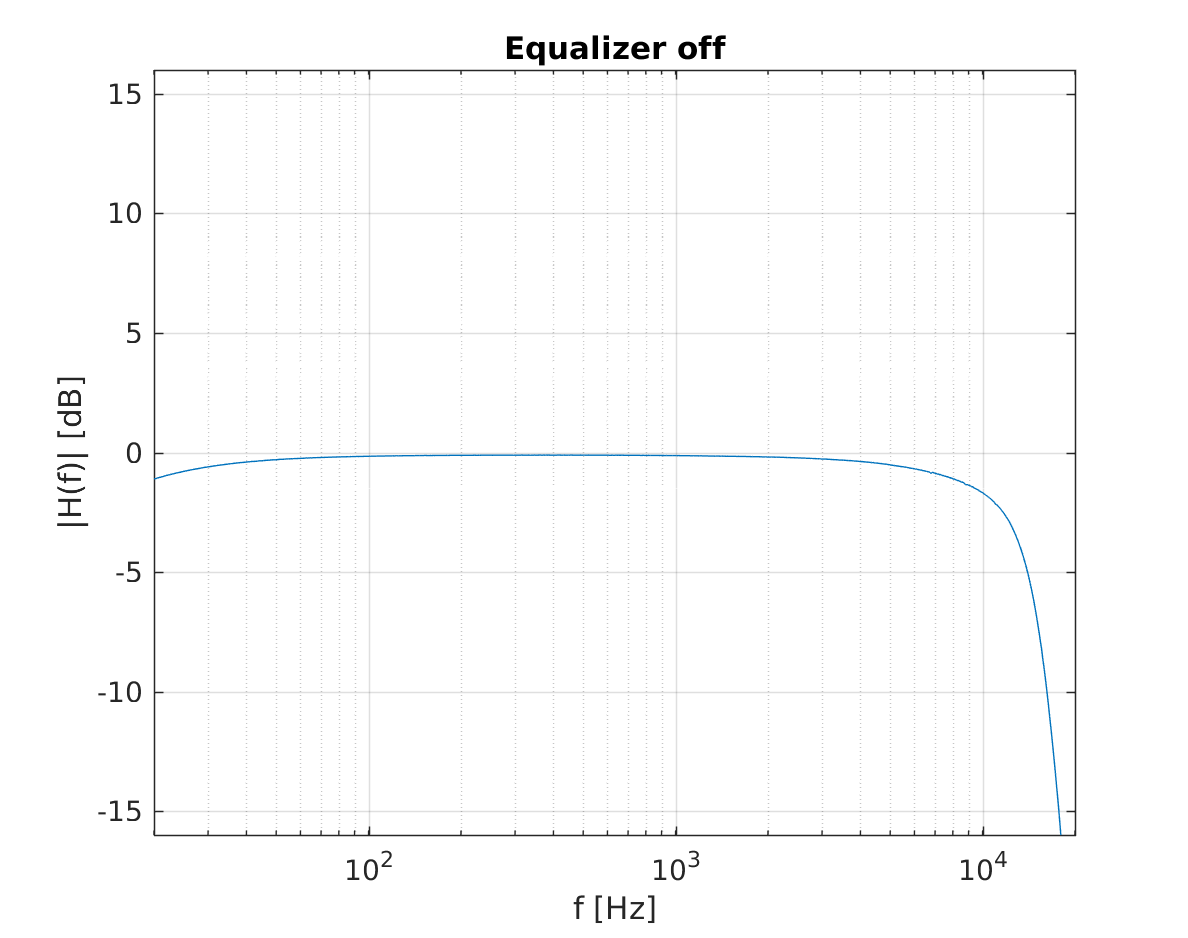
\includegraphics[]{matlabdemo/test/eq_off.png}  
%\caption{Måling af hele systemet uden equalizer slået til.}
%\end{figure}

%\begin{figure}[h]
%\centering
%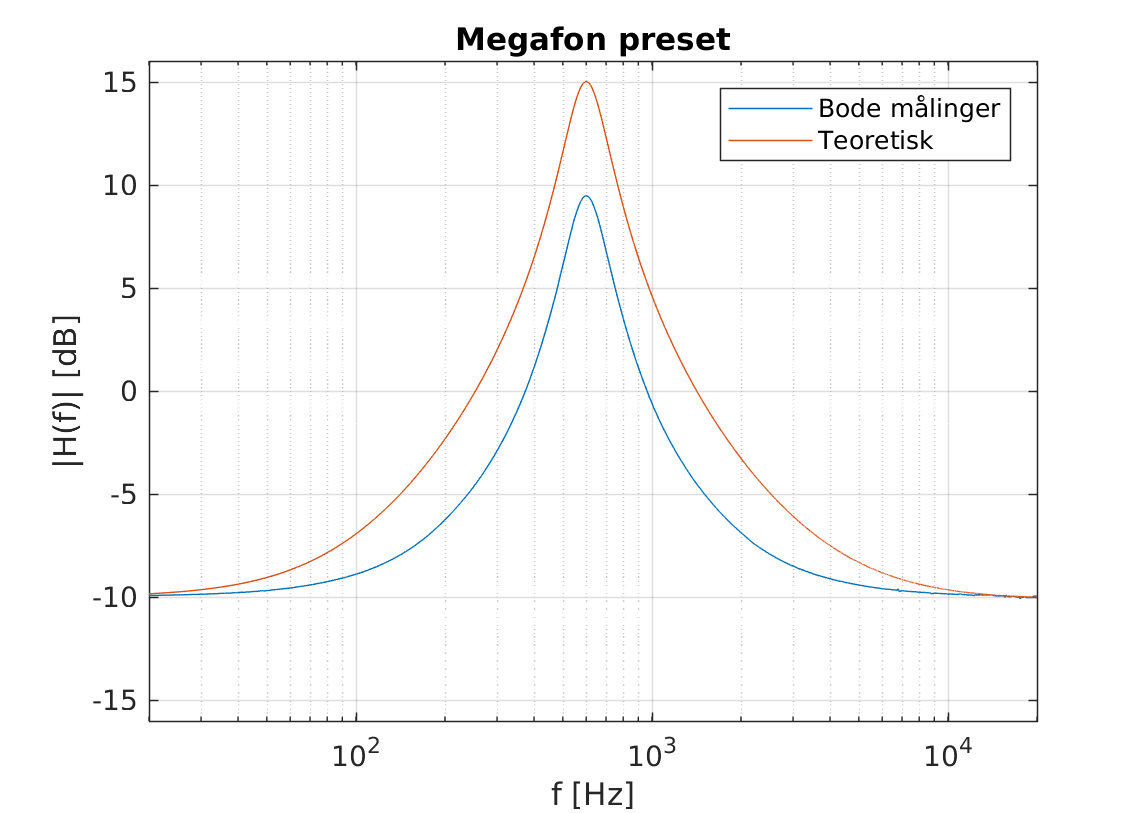
\includegraphics[]{matlabdemo/test/eq_megafon.png}
%\caption{Måling af megafon preset.}
%\end{figure}
%
%\begin{figure}[h]
%    \centering
%    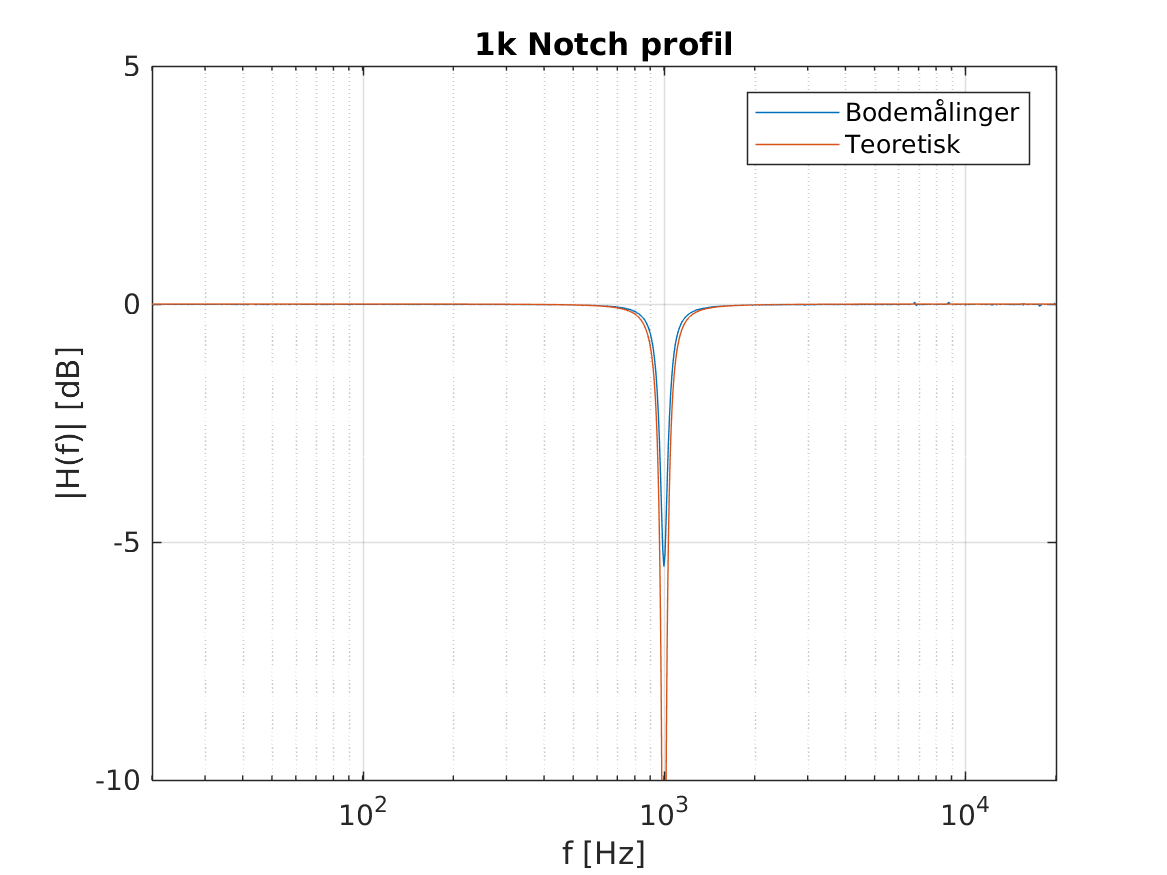
\includegraphics[]{matlabdemo/test/eq_1knotch.png}
%\end{figure}

%\begin{figure}[h]
%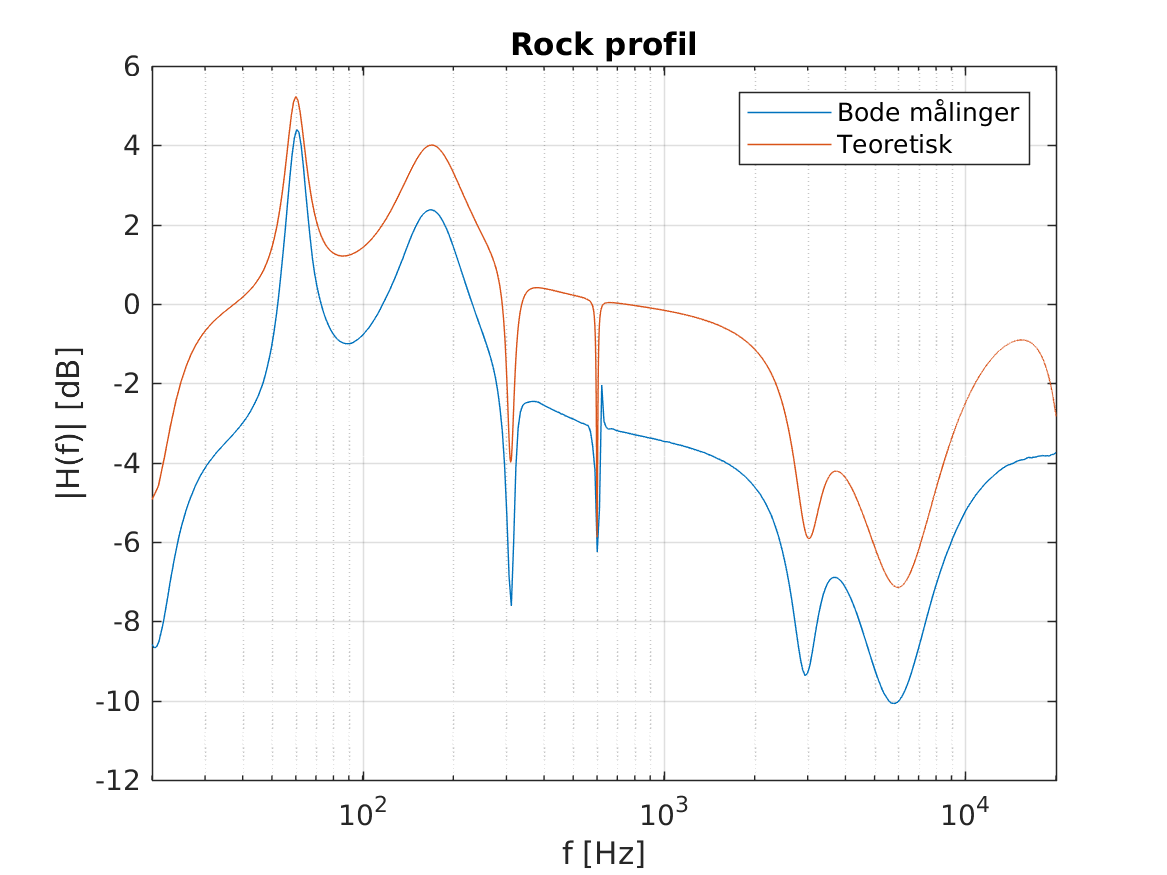
\includegraphics[]{matlabdemo/test/eq_rock.png}
%\caption{Sammenligning mellem den teoretiske rock profil og den målte.}
%\end{figure}


\begin{figure}[h!]
\centering
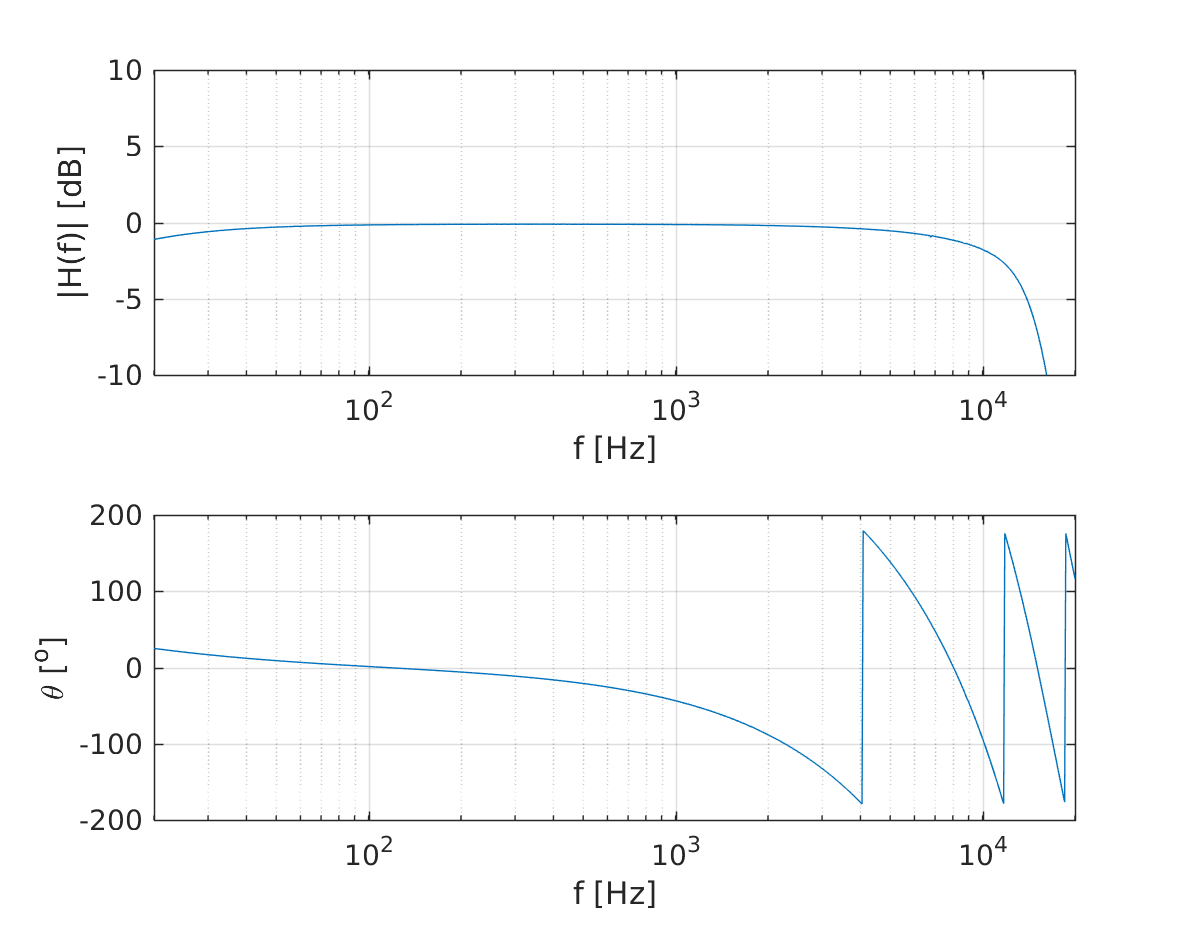
\includegraphics[scale = 0.8]{matlabdemo/test/test_eq_off.png}  
\caption{Måling af hele systemet uden equalizer slået til.}
\label{fig:eq_off1}
\end{figure}

%\subsection{Frekvensplacerings}


\begin{figure}[h!]
\centering
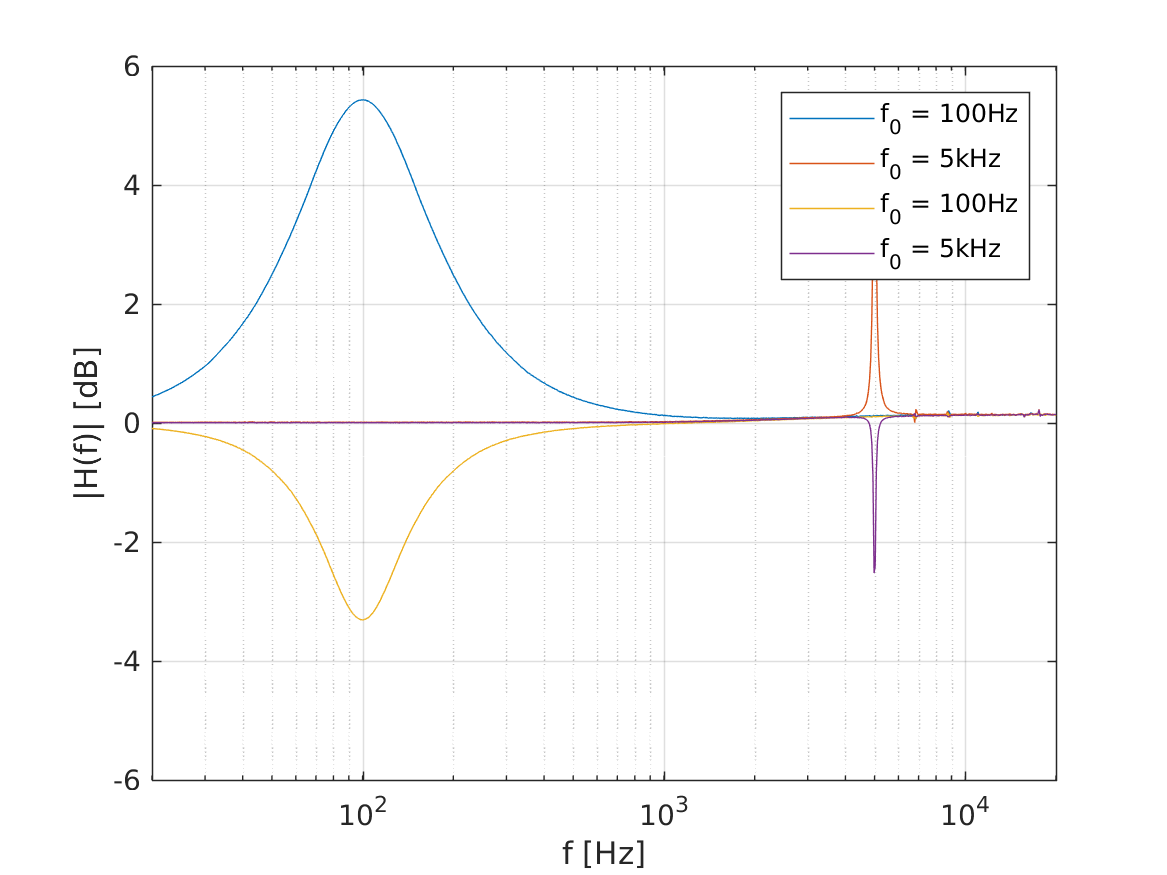
\includegraphics[scale = 0.8]{matlabdemo/test/test_freq_peak.png}
\caption{Måling af forskellige amplituder.}
\label{fig:eq_freq_peak}
\end{figure}




%\subsection{Båndbredde}

\begin{figure}[h!]
\centering
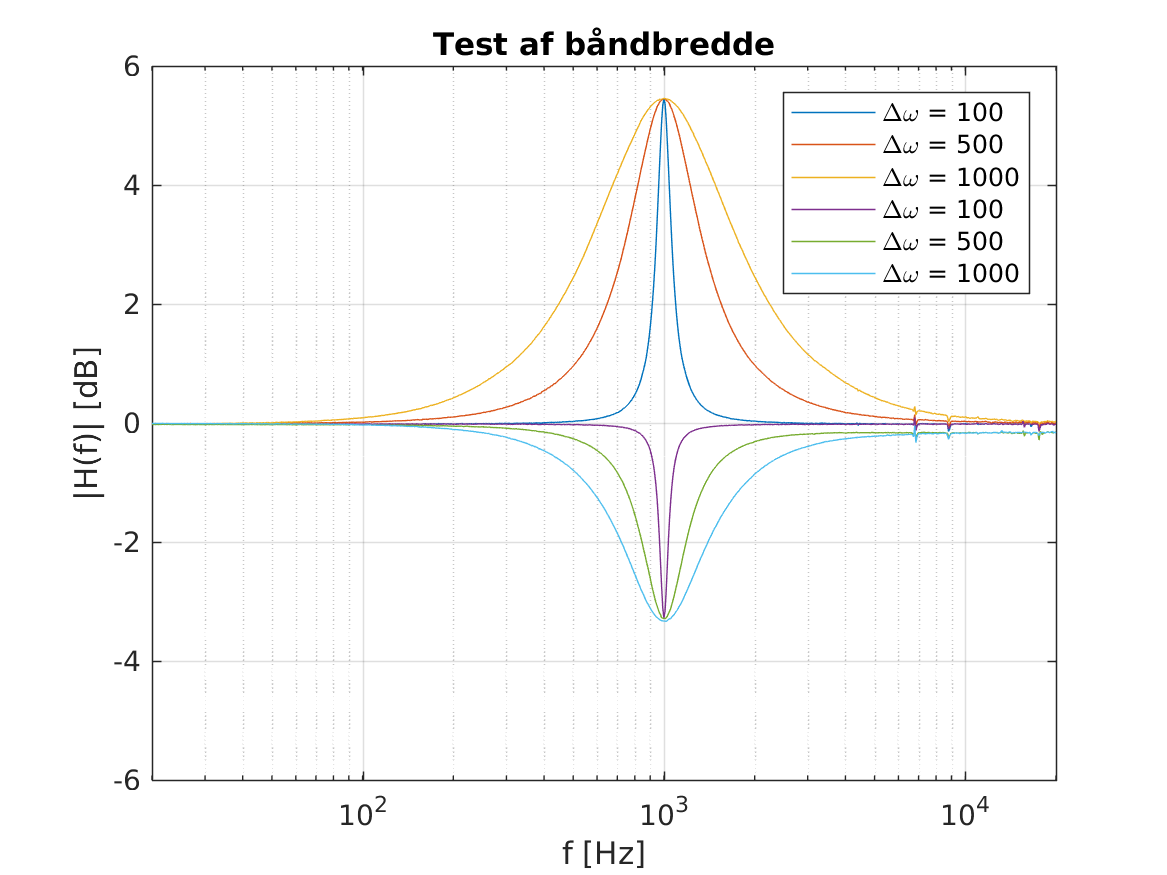
\includegraphics[scale = 0.8]{matlabdemo/test/test_bw.png}
\caption{Måling af varierende båndbredde.}
\label{fig:eq_bw}
\end{figure}




%\subsection{Amplitude}

\begin{figure}[h!]
\centering
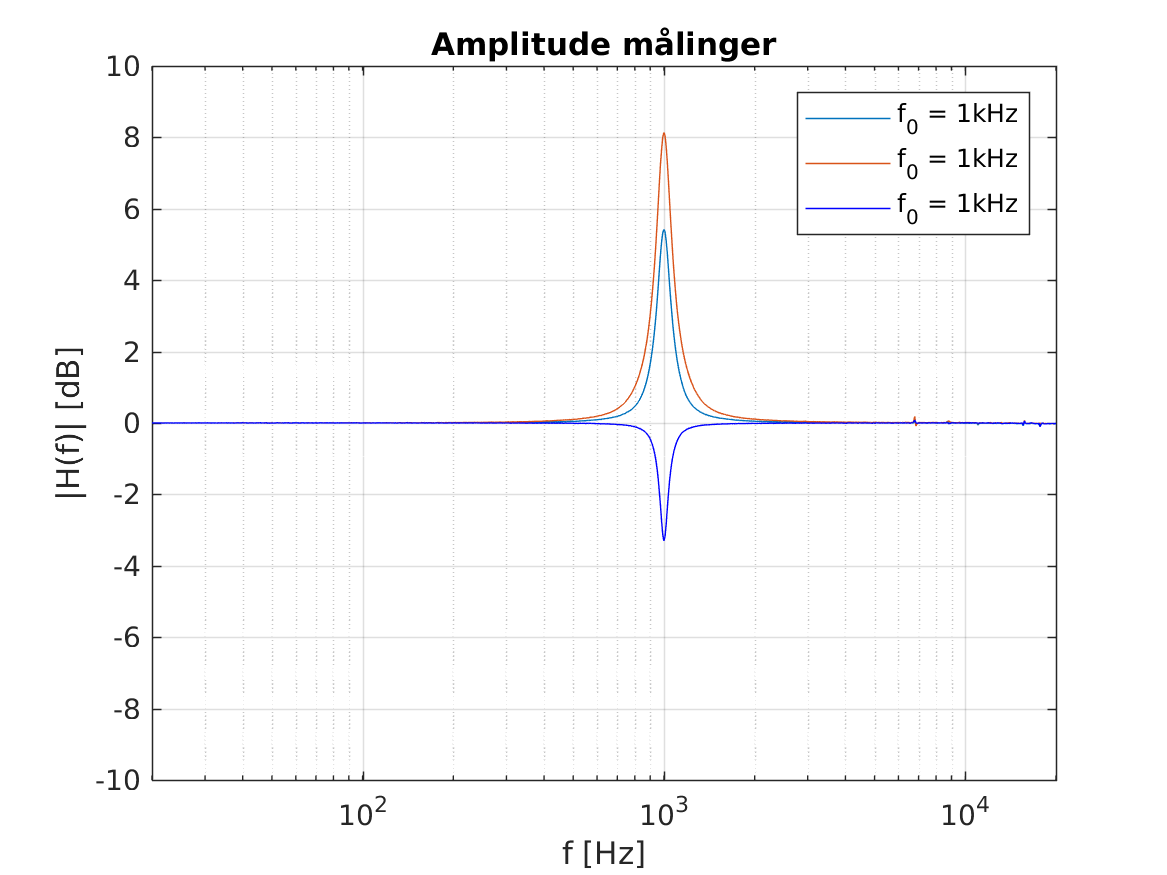
\includegraphics[scale = 0.8]{matlabdemo/test/test_amp.png}
\caption{Måling af forskellige amplituder.}
\label{fig:eq_amp}
\end{figure}


%\begin{figure}[h]
%    \centering
%    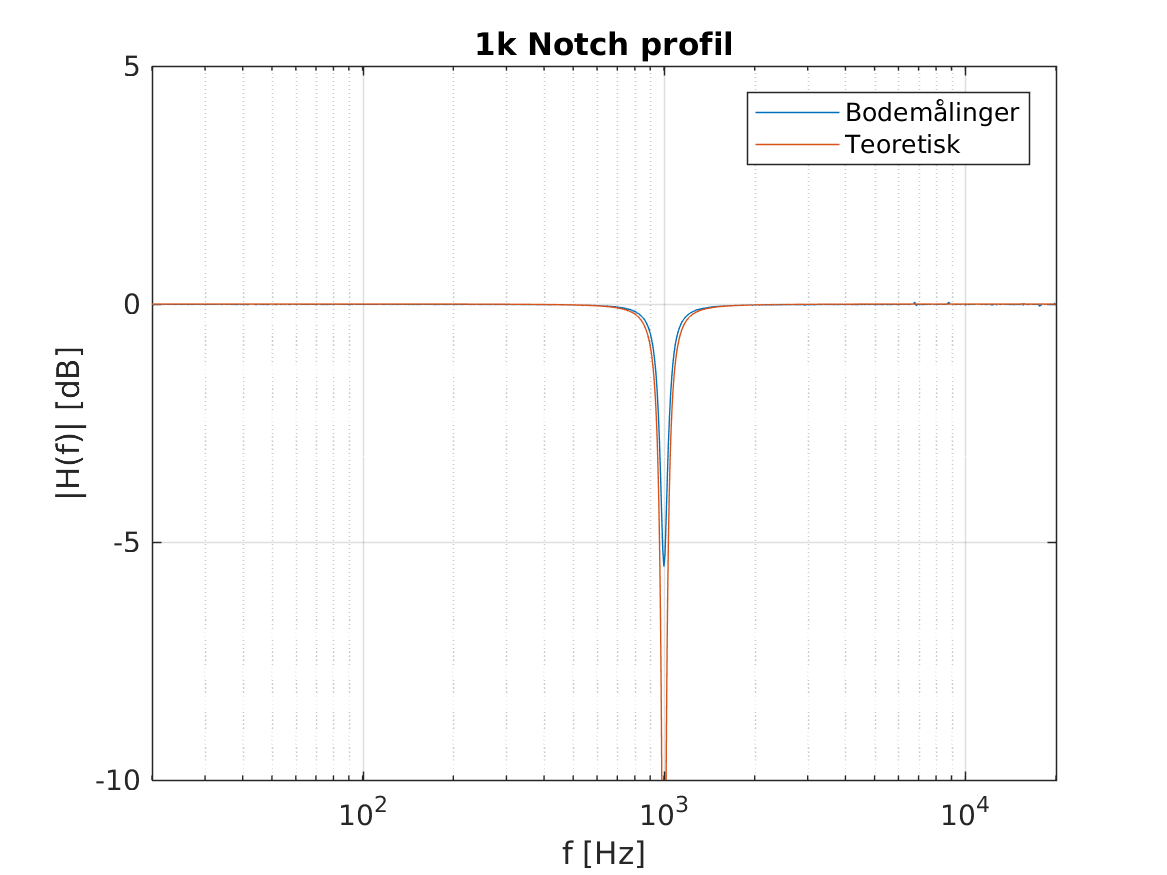
\includegraphics[]{matlabdemo/test/eq_1knotch.png}
%\end{figure}
%
%\begin{figure}[h]
%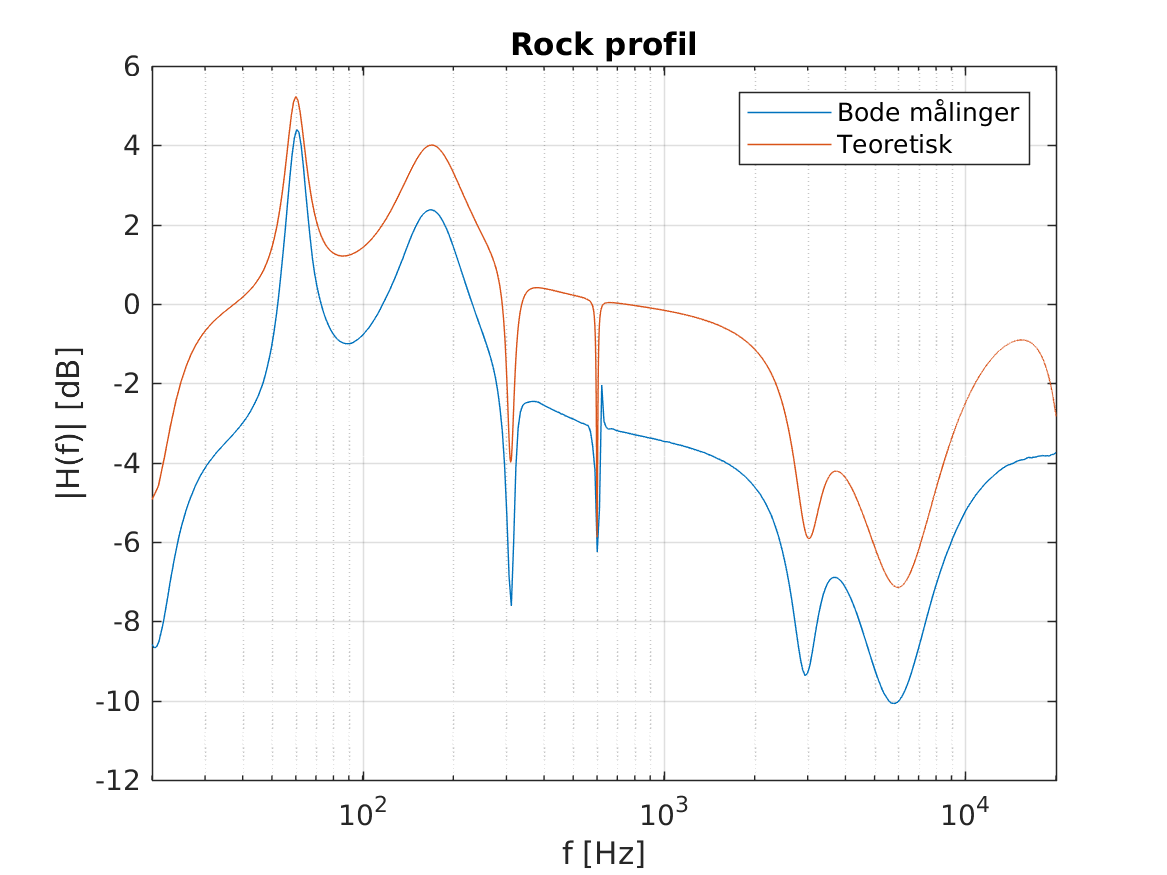
\includegraphics[]{matlabdemo/test/eq_rock.png}
%\caption{Sammenligning mellem den teoretiske rock profil og den målte.}
%\end{figure}






